
\documentclass{article}
\usepackage[utf8]{inputenc}

% Setting for formatting title page
\usepackage{titling}
\renewcommand\maketitlehooka{\null\mbox{}\vfill}
\renewcommand\maketitlehookd{\vfill\null}

\PassOptionsToPackage{hyphens}{url}\usepackage{hyperref} % URLs
\usepackage{amsmath} % For maths
\usepackage{amsfonts} % For some maths fonts e.g. double struck
\usepackage{palatino} % Font
\usepackage[margin = 3.81cm]{geometry} % Set margins
\usepackage{parskip} % Space between paragraphs

% For images
\usepackage{graphicx}
\graphicspath{{charts/}}

% Packages for tables
\usepackage{makecell} % For tables
\usepackage{multirow} % For merging cells vertically in tables
\usepackage{rotating} % For landscape tables
\usepackage{tabularx}
\usepackage{longtable}
\usepackage[flushleft]{threeparttable} % For table notes
\usepackage{threeparttablex} % For table notes in long tables
\usepackage{booktabs}
\usepackage{afterpage}

% Settings for bibliography
\usepackage[authordate, backend = biber, isbn = false, maxcitenames = 2, style = apa]{biblatex}
\addbibresource{scr-bib.bib}
\AtEveryBibitem{\clearfield{note}}

\title{Global Implications of Industrial Policies for \\ Supply Chain Resilience\thanks{I am grateful to Jason Tabarias for helpful conversations and comments and to Owen Crofts and Tisha Shah for excellent research assistance.}}
\author{Sam Hardwick}
\date{Draft, not for circulation \\ Last updated 24 September 2024}

\begin{document}

\maketitle
\begin{abstract}
    Governments are increasingly pursuing industrial policies with supply chain resilience as their stated objective. We review the theoretical grounds for such policies, their current implementation, and their governance under world trade rules. To analyse international spillovers from these policies, we present a simple three-country model with sequential production and random supply disruptions. Four simulated examples are provided: entry subsidies, production subsidies, tariffs on inputs, and export bans. Entry subsidies tend to reduce supply volatility but at relatively high cost to the subsidiser. Small production subsidies may increase global welfare but do not necessarily reduce supply volatility. Tariffs exhibit a familiar prisoner's dilemma structure. In the export ban example, the equilibrium without cooperation can be universally undesirable, in both expected value and volatility terms. We conclude by positing some rules of thumb for resilience policy, emphasising the importance of competition, appropriate instrument selection, and focusing on essential and vulnerable sectors. Internationally, we point to potential benefits from expanding data collection and independent monitoring of GVCs in critical sectors, before briefly reviewing WTO reform proposals that might better accommodate resilience concerns.
\end{abstract}

\section{Introduction}

Around the world, industrial policies have proliferated in size and number, with a particularly steep uptick among high-income countries since 2020 (Figure \ref{fig:subsidies}). This trend has coincided with and responded to a growing policy interest in supply chain resilience, reflecting supply challenges in the depths of the COVID-19 pandemic as well as security anxieties arising from great power rivalry \parencite{ilyina_industrial_2024}.

The pandemic demonstrated that global value chains (GVCs) are susceptible to disruption and that shocks to downstream or upstream sectors can reverberate throughout the chain, potentially with macroeconomic consequences. As pandemic risks have abated, geopolitical risks to supply chains have become the object of focus. Simultaneously, risks related to climate change have continued to rise.

\begin{figure}
    \caption{Subsidy policies implemented since January 2009, cumulative, by income group}
    \label{fig:subsidies}
    \centering
    \begin{minipage}{0.6\linewidth}
        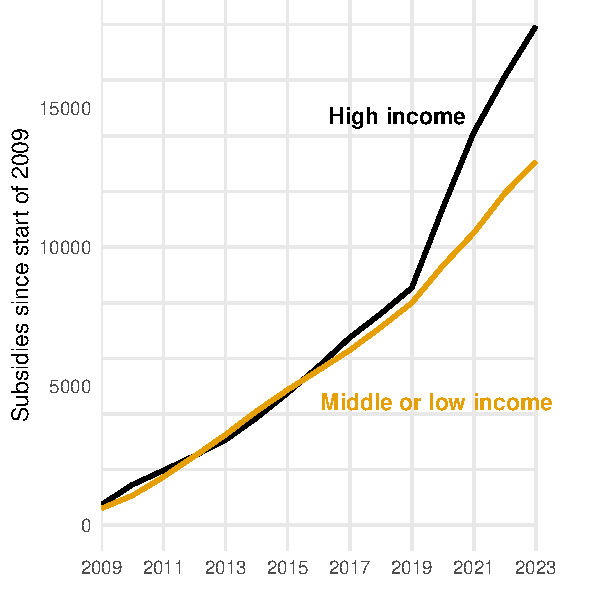
\includegraphics[width = \linewidth]{subsidies.pdf}
        \\
        \small{Source: Calculations based on Global Trade Alert (2024) data and World Bank income groups as of August 2024.}
    \end{minipage}
\end{figure}

While shocks are transmitted through GVCs, 'renationalising' these chains does not, in general, make economies more resilient to those shocks, as a major study of COVID-19 lockdowns points out \parencite{bonadio_global_2021}. Access to international trade is a buffer against domestic shocks and access to multilateral trade is a buffer against bilateral shocks. As \textcite{caselli_diversification_2020} argue, in the presence of country-wide shocks, openness lowers volatility by allowing diversification of supply and demand. Their results indicate that this has been the case for most countries in recent decades. In a more immediate sense, the astonishing rebound of global merchandise trade in 2021 and early 2022 suggests that GVCs were more resilient than they may have appeared.

Research since the pandemic has also pointed to conditions in GVCs or supply networks that can give rise to market failures or that amplify economic shocks. Some structures of supply networks are more fragile or transmit shocks more quickly than others \parencite{elliott_networks_2022}. The entry of new firms in a network prone to disruption is a positive externality, in terms of risk reduction, that markets may fail to price in \parencite{bimpikis_supply_2019}. `Bottleneck firms' might systematically underproduce inputs, and regulatory or informational barriers might discourage efficient investment in risk management \parencite{carvalho_supply_nodate, productivity_commission_vulnerable_2021}. 

With notable exceptions like the work of the \textcite{productivity_commission_vulnerable_2021} and \textcite{grossman_supply_2023}, economic research on supply chain resilience has tended not to address questions of optimal public policy, beyond sometimes pointing to a general role for it.\footnote{\textcite{grossman_supply_2023} identify a business-stealing externality, where a firm's profits, if they avoid supply disruption, come at the expense of other viable firms without creating new value. If this effect---which gives rise, perhaps counterintuitively, to \textit{over}investment in resilience---dominates other externalities, overall welfare is reduced. The authors show that government can achieve efficient sourcing with a combination of product-specific consumption subsidies and diversification taxes.}

As this literature has grown, so has the footprint of industrial policies on the global economy. It is evident that subsidies, first-best or otherwise, will play a central role in the green energy transition, a phenomenon which is reorganising GVCs. These developments have intensified interest in supply chain resilience and industrial policy as governments seek both energy security and market shares in the future low-carbon global economy. This economy demands inputs, not just critical minerals but also manufactured goods, that today may be concentrated in relatively few hands.

The desire for diversification has been a stated motive for recent industrial policies in some countries, often on national security grounds. But diversification, though related to resilience, is not equivalent to it, particularly if diversifying means sacrificing optimal technology, comes at the price of other productive activities, or is pursued in a way that raises trade uncertainty or sparks retaliation. Likewise, the impacts of industrial policies on supply chain resilience are not clear cut. There are negative and positive spillovers to consider, domestically and globally. A central question, posed by \textcite{bown_modern_2024}, is whether optimal supply chain resilience policy from a domestic standpoint differs to that from a global standpoint.

To contribute to answering that question, and to better understand these policies and spillovers, we proceed as follows. The next section reviews the theoretical bases for policies to manage supply chain risk, which policies countries are using, and how these policies are governed in the world trading system. We then present a simple three-country model with sequential production and random supply disruptions to explore these policies and illustrate their potential international spillovers. As performance indicators, we look both at conventional measures of economic welfare as well as the variation of final supply of a product. We simulate four policy examples targeting upstream inputs: entry subsidies, specific production subsidies, import tariffs, and export bans.

The policy examples reflect and extend findings from trade policy models without disruption risk. Subsidies that target entry costs alone preserve the international composition of production while encouraging new firms, thus reducing disruption risk, though at a large cost to the subsidiser. Small production subsidies can increase global welfare and supply---most effectively if applied in tandem rather than unilaterally---though they do not make final supply less volatile. Tariffs exhibit a familiar prisoner's dilemma game, pointing to a non-cooperative equilibrium that lowers welfare and supply without offering reduced volatility of consumption. The prospect of export bans to reduce the probability of a downstream shortage can elicit a globally inefficient equilibrium in the absence of cooperation.

In light of these examples, we conclude by discussing some emerging rules of thumb for domestic supply chain resilience policy, and by reviewing active policy proposals for international cooperation in that domain. Finally, we suggest directions for future research.

\section{Industry policy, supply chain resilience and the world trading system}

\subsection{For and against industrial policy for supply chain resilience}

Though in many respects, GVCs fared remarkably well through the pandemic, several experiences in recent years have led policymakers to question the adequacy of status-quo approaches to supply chain risk. The most severe examples were the shortages of personal protective equipment in many jurisdictions. Shortages of diesel exhaust fluid (DEF) in 2021 were another. A perfect storm of global influences, chiefly food price inflation, rebounding energy demand and fertiliser export controls, saw exports of technical-grade urea---the main input to DEF---dry up, seriously threatening internal freight in countries like the Republic of Korea and Australia. 

Against the backdrop of the pandemic, countries initiated, in the name of supply chain resilience, grant programs, strategic industrial plans, on-shoring subsidies, bilateral dialogues and domestic advisory bodies. They imposed trade restrictions, created or expanded critical minerals lists, launched infrastructure programs and announced regional supply chain initiatives. The Indo--Pacific Economic Partnership (IPEF), launched in May 2022, took on supply chains as one of its four foundational pillars \parencite{hardwick_policy_2024}.

Following \textcite{harrison_trade_2010} and \textcite{bown_modern_2024}, this paper defines industrial policy in broad terms as deviation from policy neutrality. While we focus our analysis on more conventional industrial policies, others like trade agreements, commercial diplomacy, competition policy and regulatory reform are essential to the resilience toolkit. Lowering barriers to entering domestic or foreign markets expands the scope of risk management strategies available.\footnote{See \textcite[145--148]{productivity_commission_vulnerable_2021} on the role of an open trading environment in managing supply chain risk.}

There are several well-known economic arguments for industrial policy. Sometimes these arguments are based on internal economies of scale, such as learning by doing that occurs within a firm. More commonly, arguments refer to externalities. Benefits from technological development, knowledge generation or human capital advancement in one firm can spill over to others. In recent decades, more emphasis has been placed on industrial policy's role in discovering the costs and benefits of new economic activities, and in addressing coordination issues through public--private cooperation \parencite{rodrik_industrial_2004}.

In the subdomain of supply chain resilience, there are further arguments for industrial policy, defined in this broad sense. All organisations and GVCs face some level of disruption risk, which can be thought of as the likelihood of some event that directly affects its usual functioning---its ability to deliver `the right products and services on time, with the required specifications, at the right place and to the right customer' \parencite{carvalho_supply_2012}. Following \textcite{baldwin_risks_2022}, we can think of socially excessive risk as a situation where firms' decisions lead to a different bundle of risk and reward---reward such as cost savings---than what public interest would demand. Socially excessive supply chain risk can be a symptom of traditional market imperfections. For example, industries with few new entrants are more likely to see bottleneck firms emerge \parencite{carvalho_supply_nodate}, which wield market power, restrict supply and concentrate risk.

A key example of potentially excessive supply chain risk is that modelled by \textcite{bimpikis_supply_2019}. The authors show that, under certain conditions, the equilibrium number of entrants in a supply network may be lower than the number that maximises consumer surplus and profit. In an environment where firms face random disruptions, new firms, through the act of entry, benefit the rest of their supply network by diversifying supply or demand. Firms might be able to reap \textit{some} of these external benefits---by profiting off their reputation as reliable suppliers, for example---but not all of them, without implausibly sophisticated contracting across all firms in a network.\footnote{Other potential sources of socially excessive risk are reviewed by \textcite{elliott_networks_2022} and \textcite{hardwick_policy_2024}.} 

Conversely, there are areas where exposure to supply chain risk may appear high, but there is no clear policy rationale for addressing it directly. For example, in some cases, there is a trade-off between a lengthy, high value-adding GVC and a shorter, more expensive, less volatile one \parencite{levine_production_2012}. Some network structures have been shown to propagate shocks more intensely than others \parencite{todo_propagation_2019}. Yet there is no case in principle for intervention unless that intervention might be expected to bring about a socially superior balance of risk. As \textcite[3493]{grossman_supply_2023} put it, while commentators have been quick to conclude governments should take a stronger role in promoting resilience, the welfare calculus around intervention is `subtle', and only `when the private incentives for resilience fall short of the social benefits will government encouragement be warranted.'

On that basis, as the Australian \textcite{productivity_commission_vulnerable_2021} has outlined, policies to improve supply chain resilience are best targeted at vulnerable and essential products, where public risk appetites are lowest. `Essential' may sound like a slippery concept, but it is one that governments regularly deal with; for example, in strategising for disaster management or maintaining pharmaceutical or energy stockpiles. As vulnerability (or exposure to risk) and essentiality decline, private risk management is more likely to suffice. In addition to vulnerability and essentiality, the \textcite{productivity_commission_vulnerable_2021} include a third criterion, criticality, or how difficult it is to substitute a given input for another.

The role of entry barriers in generating excessive supply chain risk suggests that industrial policy is more likely to aid resilience if it permits or encourages competition. A corollary is that policies are more likely to reduce resilience if they limit competition, either by restricting entry or favouring non-competitive incumbents. Empirical studies of industrial policy more broadly suggest competition is a critical variable. Evidence from China indicates that subsidies to more competitive sectors are most likely to boost productivity, while those to less competitive sectors tend to reduce it \parencite{aghion_industrial_2015}. In Japan, the sectors that benefited from industrial policy in the 1970s, 80s and 90s succeeded internationally if there was a high level of domestic competition \parencite{porter_competition_2004}.\footnote{\textcite{studwell_how_2014} explores this theme in depth for the East Asian region.}

Concentration of production by country is a flawed but sometimes informative proxy for competition issues that may present vulnerability. Concentrated production does not inherently mean there are barriers to entering and producing. It may be a temporary but desirable result of a firm or set of firms innovating. In some cases, however, concentration may be a signal of vulnerability to shocks---the key variable being whether alternative suppliers can enter or scale up quickly enough to deliver the socially optimal response if the main source is disrupted. Action to reduce this kind of risk may take the form of diversification, including through subsidies or agreements with third countries, or other risk management strategies, like emergency stockpiling or data sharing.

The choice of instrument matters and depends on institutional context. Subsidies and trade levers, though still common (Figure \ref{fig:instruments}), are not the only tools available. Other industrial policy tools, such as infrastructure investment, manufacturing extension and specialised training, may better serve both competition and productivity goals \parencite{juhasz_new_2023}. A survey of 50 years of US industrial policies points to research and development (R\&D) programs as having by far the best track record of any instrument \parencite{hufbauer_scoring_2021}. The authors also conclude that import protection rarely achieved its stated aims, except for when it successfully induced a world-class firm to relocate to the tariff-imposing country.\footnote{Toyota in the 1980s is presented as an example \parencite{hufbauer_scoring_2021}} Trade agreements, commercial diplomacy and regulatory reform may all be beneficial for supply chain resilience to the extent that they address barriers to alternative sources of supply and demand.\footnote{See \textcite{fry-mckibbin_does_2019} for empirical evidence on the ability of commercial diplomacy to address informational and regulatory barriers to trade.} Sometimes more security-focused policies like stockpiling may be reasonable alternatives, if storage and other costs are low enough.\footnote{By way of example, the Australian government's response to DEF shortages was ultimately a combination of stockpiling, grants for sovereign capability, and greater industry data collection (DCCEEW, 2024).}

\begin{figure}
    \caption{Number of interventions by instrument in Global Trade Alert database, 2009--2023}
    \label{fig:instruments}
    \centering
    \begin{minipage}{0.6\linewidth}
        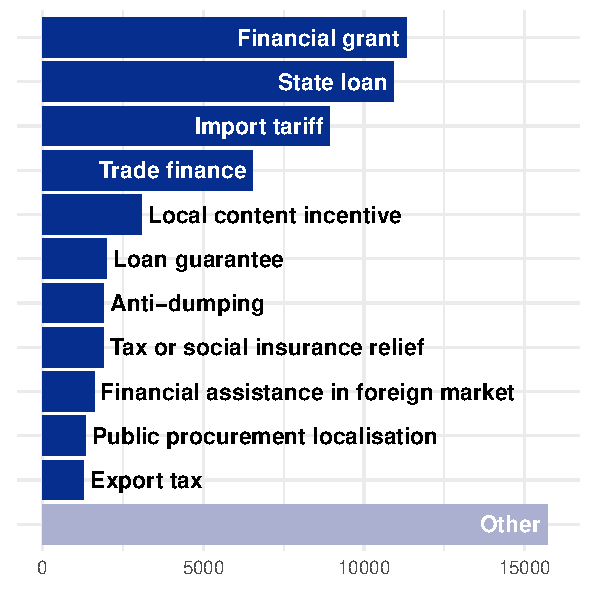
\includegraphics[width = \linewidth]{instruments.pdf}
        \\
        \small{Source: Authors' calculations based on Global Trade Alert (2024) data.} 
    \end{minipage}
\end{figure}

Industrial policies have positive and negative international spillovers for supply chain resilience. On the positive side, industrial policies may accelerate the development of technology which, with sufficient factor mobility, spreads internationally. They may facilitate new exporters, diversifying the supply or customer base. On the negative side, they may erode international competition, including by limiting export-competing countries’ access to third markets. These effects lower resilience by limiting the ability of new supply to enter. They may lead to wasteful subsidies races: if one country subsidises, its competitor may be forced to subsidise too or exit markets.

Beyond subsidies, other policy instruments may have more direct implications for supply chain resilience. Local content requirements may impede responses to shocks by removing alternative supply options, or at least by delaying the ability to adjust. Export bans similarly remove an input source from global markets. Cooperation is needed to identify and measure these spillovers to inform multilateral subsidy rules, especially where trade and climate change imperatives interact \parencite{bown_modern_2024}.

\subsection{Supply chain resilience policy and multilateral trade rules}

Current world trade rules and regional arrangements offer frameworks for managing some of these spillovers, but there are widely held doubts about their adequacy in addressing contemporary challenges. There have long been diverse perspectives on how the WTO may be best reformed to deal with subsidies, with some scholars advocating for more flexibility and others emphasising better definition and reporting and sharper disciplines, each with the goal of restoring the system. China's pivotal position in GVCs and the massive, complex role of the state therein has intensified these debates.

The origins of the world trading system are deeply intertwined with concerns about the security of supply and its global strategic implications. One of the Atlantic Charter's eight clauses concerns the access of all nations to trade and raw materials necessary for prosperity. This vision materialised in the GATT and carried through to the creation of the WTO. Yet the objectives of prosperity and security are today increasingly viewed in zero-sum terms \parencite{armstrong_economics_2023}, and the current state of the world trading system is marked by deadlock. The question of whether reform can proceed through multilateral channels depends on what reforms are actually desirable, especially to address challenges like climate change.

Most proposals for moving world trade rules forward against this backdrop is to do so through plurilateral channels, including WTO plurilaterals, and possibly through separate agreements between major economies in domains like the green energy transition. As \textcite{bown_how_2023} outline, an agreement between the United States, China and the European Union could accommodate certain industrial policies for a green economy while agreeing to refrain from others, such as export restrictions. Forums like APEC or the RCEP economic cooperation agenda could present similar pathways in a regional context.

The WTO governs subsidies primarily through the Agreement on Subsidies and Countervailing Measures (ASCM), which defines a subsidy as a `financial contribution' by a government or `public body' that confers a benefit. The agreement categorises subsidies into prohibited (namely export and local content subsidies) and actionable subsidies that cause adverse effects to other members. For the latter, the agreement offers two remedies: countervailing duties that can be imposed on subsidised imports causing injury to domestic producers; and dispute settlement, usually if the adverse effects are from displacing exports in the subsidising market or a third market. Members are required to notify the WTO of their subsidies but compliance with this requirement has been poor \parencite[570]{bown_wtoing_2019}. The ASCM only covers subsidies that are `specific', either by firm, industry or region, or those that target exports.

There is a wide range of views on how subsidies should best be handled by multilateral trade rules. At one end, \textcite{sykes_subsidies_2005, sykes_questionable_2010} argues the best approach to subsidies in the WTO may be, with the exception of the non-violation doctrine, an essentially laissez-faire one, given the difficulties of properly identifying subsidisation and of disentangling socially beneficial measures from protectionist ones. \textcite{bagwell_will_2006} also point to flaws in WTO subsidy rules, in contrast to those of the GATT, on the grounds that they risk undermining tariff negotiations as the primary mechanism for expanding market access. \textcite{hoekman_rethinking_2020} highlight the need for an international work program on to identify common principles, such as citizen welfare as an objective, and develop simple, robust rules of thumb for subsidies governance.

\textcite{bown_wtoing_2019}, writing about China’s industrial policy, point out that work on measurement and identification of subsidies is critical for adequate governance and reform, given the high evidentiary burden for proving that subsidies exist. Beyond that, a ‘green, amber, red light’ system would be ideal, possibly with an expanded set of prohibited subsidies.\footnote{The `green light' system would follow the 1995 WTO Agreement on Agriculture, which temporarily introduced it. \textcite{aguayo_ayala_preserving_2005} offered an early proposal to revive this system.} The authors also raise an alternative approach of introducing competition policy concepts to the WTO; for example, requiring notifications on size and competition among large firms.

It is not surprising that much of this debate focuses on China, as state-owned enterprises are controversially exempt from the official definition of `public body' \parencite[567]{bown_wtoing_2019}. A pioneering empirical study of industrial policy's foreign spillovers is that of \textcite{barwick_chinas_2019} who look at China's shipbuilding subsidies. While the net global benefits from cheaper shipping may be ultimately positive, about three-quarters of China's expanded market share during its subsidy programs came from edging out Japanese and Korean firms---and the programs had decidedly mixed results for China itself. Another example, relevant to supply chain resilience, is solar photovoltaic (PV) cell production. By 2015, thanks in significant part to industrial policy, China had become the world’s top PV cell producer. There have been large, clear positive impacts on emissions reduction and innovation \parencite{xu_impact_2022}. At the same time, overcapacity issues, coupled with high concentration at firm and facility levels, have led to concerns about global solar PV supply chain risk \parencite{wang_why_2014, iea_solar_2022}.

An interesting comparison is with Denmark's use of industrial policy to become the world leader in wind power generation technology. Denmark began producing wind turbines in the 1980s, initially supported by price guarantees and favourable tax treatment, though not by trade restrictions. Studies suggest the subsidies enabled learning by doing, with benefits that likely exceeded future discounted costs \parencite{hansen_establishment_2003}. Danish technology and knowhow ultimately spread internationally, notably through direct investment in Spain and Germany. Despite initially high concentration---Denmark accounted for over 90 per cent of global wind turbine exports in 2002---and overcapacity issues, concerns about competition and supply chain risk were muted. Few in hindsight would consider Denmark's policy-driven dominance of the sector to be a global public bad.

The question of which policies, under which underlying conditions, should be expected to generate net global benefits depends on the balance of the international spillover effects. Better understanding of these effects would therefore inform how world trade rules should address supply chain resilience policies. Spillovers are often ambiguous and always multidimensional, with global welfare comprising the expected net pecuniary costs, the net supply chain risk, and (though out of scope for this paper) the environmental effects. The next section presents a simple model to illustrate some of these spillovers.

\section{A model of trade with input disruptions}

The model below serves to illustrate potential spillovers from industrial policies for supply chain resilience by providing stylised examples. The aim is not to present sweeping policy conclusions but to highlight some mechanisms through which one country's policies might help or harm others' resilience, and areas where international cooperation may be needed to avoid lose--lose outcomes. It also provides a novel approach to integrating stochastic supply chain risks into simple trade policy models, one which may be generalised and adapted to other policy tools and scenarios.

The model has two sectors, an input $I$ and a final good $F$, and three countries, $A$, $B$ and $C$. We use three countries as two-country models miss some of the potential negative international spillovers from subsidies \parencite{bown_wtoing_2019}. One country's subsidies can carve out a competitor's market share in a third country to which they both export. Here, $C$ does not produce either good, but represents the third market where $A$ and $B$ compete, thereby capturing some of these spillovers. 

The model proceeds as follows. First, firms decide whether or not to enter the market for inputs. In doing so, they consider the prices they will face, which depend on policies, their risk of a disruption, the costs of trade and the price of raw materials. They also consider consumers' demand for the final product, which depends on incomes and the elasticity of substitution between domestic and foreign goods. To enter the market, they need to pay an entry cost $\kappa$ and purchase raw materials on a global exchange at price $p_r$, taken as given. If their expected profits are positive, they will enter.

Once they have entered, whether or not they produce and sell inputs depends on a stochastic disruption risk, $d_j \in (0, 1)$. A firm in country $j$ will make inputs with probability $1 - d_j$, but if it is disrupted, it will not produce and the raw materials it purchased will be wasted. This process echoes the model of \textcite{bimpikis_supply_2019}.

After the entry process, prices are considered set, and production occurs. Input producers purchase raw materials and either make inputs or experience a disruption. The inputs are sold to firms in the final good sector in countries $A$ and $B$, transformed into final goods, then sold to customers in countries $A$, $B$ and $C$. Welfare is evaluated based on consumption of the final good and income after any revenue from tariffs or costs of subsidies have been accounted for.

The model draws on that of \textcite{melitz_missing_2014}, who outline a simple model of sequential production that shows how trade can increase domestic productivity as the number of production stages increases. The setup and representation of profits are also similar to those of \textcite{venables_trade_1987} and \textcite{bagwell_design_2016}.

\subsection{Consumers}
 
Each country $j$ has a representative consumer with constant elasticity of substitution (CES) preferences. These consumers maximise utility given by
\begin{equation}
    U_j = \left[ (x_{FAj})^{\frac{\sigma - 1}{\sigma}} + (x_{FBj})^{\frac{\sigma - 1}{\sigma}} \right]^{\frac{\sigma}{\sigma - 1}}
\end{equation}
where $x_{Fij}$ represents consumption in country $j$ of final goods produced by country $k$. The elasticity of substitution between goods from different countries is $\sigma > 1$. Consumers face the budget constraint 
\begin{equation}
    p_{FA} \bar{\tau}_{FAj} x_{FAj} + p_{FB} \bar{\tau}_{FBj} x_{FBj} \leq M_j
\end{equation}
where $p_{Fi}$ is the price of final goods produced in country $i$ and $M_j$ is income in country $j$. $\bar{\tau}_{Fij}$ captures trade costs faced by importers from $j$ of final goods from $i$. This term takes the value 
\begin{equation} \label{eq:tau}
    \bar{\tau}_{Fij} =
    \begin{cases}
        1 &\text{if } i = j \\
        (1 + t_{Fj})(1 + \tau) &\text{if } i \neq j
    \end{cases}
\end{equation}
where $t_{Fj}$ is the import tariff rate in country $j$, if one applies, and $\tau$ is a generic international trade cost, like freight. 

As shown by \textcite{dixit_monopolistic_1977}, a price index for final goods consumed in country $j$ can be defined as
\begin{equation} \label{eq:pbar_f}
      \bar{P}_{Fj} = \left[ (p_{FA} \bar{\tau}_{FAj} )^{1-\sigma} +  (p_{FB} \bar{\tau}_{FBj})^{1-\sigma} \right]^\frac{1}{1-\sigma} .
\end{equation}
Using the price index in (\ref{eq:pbar_f}), demand for final goods produced in country $k$ and consumed in country $j$ can be written as
\begin{equation}
    x_{Fij} = M_j \left( \frac{p_{Fij}}{\bar{P}_{Fj}} \right)^{-\sigma}  .
\end{equation}
For simplicity, we assume the elasticity is constant across all stages of production, though it could be allowed to vary. Our baseline considers an elasticity $\sigma$ equal to 5. A comprehensive survey of Armington elasticities posits a `best guess' of the range of empirical estimates at 2.5 to 5.1 with a median of 3.8 \parencite{bajzik_estimating_2020}. A value at the high end of that range was selected because we are interested in relatively specific, relatively similar varieties across the two countries.\footnote{While we do not include a sensitivity analysis here, a draft version of the model code is \href{https://github.com/sjhardwick/supply_chains}{available on GitHub}.}

Welfare is evaluated using the indirect utility function
\begin{equation} \label{eq:value}
    V_j = I_j \bar{P}_{Fj}
\end{equation}
where $I_j$ equals $M_j$ plus any net revenue from tariffs, costs from subsidies, and any profits in the input sector in country $j$. The final goods sector makes zero profit.

\subsection{Final good sector}

The final good sector consists of a single representative firm per country, one in country $A$ and one in country $B$. Country $C$ consumes final goods but does not produce them. Since we are interested in market imperfections upstream---supply chain disruptions---we assume perfect competition in the final good sector. Each firm in the sector sources a mix of domestic and foreign inputs and produces according to CES technology, given by
\begin{equation} \label{eq:prod_final}
    Q_{Fj} = \left[ \left( x_{IAj} \right)^\frac{\sigma-1}{\sigma} + \left( x_{IBj} \right)^\frac{\sigma-1}{\sigma} \right]^\frac{\sigma}{\sigma-1}
\end{equation}
where $x_{Iij}$ are inputs sourced by country $j$ from country $i$ for production of goods $Q_{Fj}$. 

They sell these goods to consumers in the three countries. The firms' production costs are
\begin{equation}
    C(Q_{Fj}) = p_{IA} \bar{\tau}_{IAj} x_{IAj} + p_{IB} \bar{\tau}_{IBj} x_{IBj}
\end{equation}
where input trade costs $\bar{\tau}_{Iij}$ capture any tariffs and transport costs and are defined analogously with those in (\ref{eq:tau}).

With perfect competition and constant returns to scale, price $p_{Fj}$ is equal to unit cost. We can also express this unit cost as a price index $\bar{P}_{Ij}$ for inputs, that is,
\begin{equation}
    \bar{P}_{Ij} = p_{Fj} = \left[ ( p_{IA} \bar{\tau}_{IAj} )^{1 - \sigma} + ( p_{IB} \bar{\tau}_{IBj} )^{1 - \sigma}) \right]^{\frac{1}{1 - \sigma}}
\end{equation}
with conditional demand for inputs then given by
\begin{equation} \label{eq:input_demand}
    x_{Iij} = Q_{Fj} \left( \frac{p_{Ii}}{\bar{P}_{Ij}} \right)^{-\sigma}.
\end{equation}

\subsection{Input sector}

Firms in the input sector procure raw materials, which are traded freely on a global commodity market at the price $p_r$. They transform these materials directly into inputs unless they experience a disruption. The probability of a disruption for firms in country $i$ is the parameter $d_i \in (0, 1)$. Other than disruption risk, which varies by country, input-producing firms face identical technologies and costs.

Each firm's expected production can be written as
\begin{equation}
    \mathbb{E} (q_{Ii}) = (1 - d_i) r_i
\end{equation}
where $r_i$ is the quantity of raw materials purchased by each firm. Prospective input producers decide whether to enter the market based on expected profits, which are given by
\begin{equation} \label{eq:input_profit}
    \mathbb{E} (\pi_{Ii}) = \max_{p_{Ii}} \left\{ (p_{Ii} + s_{Ii}) (1 - d_i) r_{i} - p_r r_i - (1 - e_i) \kappa \right\}
\end{equation}
where $s_{Ii}$ is an optional specific production subsidy, applied per unit of input produced by firms in country $i$. $e_i$ is the rate of an optional entry subsidy and $\kappa$ represents a fixed barrier to entry. Once firms purchase raw materials, the materials may be used for production, but if there is a disruption, production cannot occur and the materials are sunk costs.

Because the total quantity of inputs produced by country $i$ equals the sum of $x_{IiA}$ and $x_{IiB}$, we can substitute the conditional demands in (\ref{eq:input_demand}) into the expected profit function in (\ref{eq:input_profit}). Doing so and solving for the profit-maximising price, assuming that producers take price indexes as given, yields
\begin{equation}
    p_{Ii} = \frac{\sigma}{\sigma - 1} \left( \frac{p_r}{1 - d_j} - s_{Ii} \right) .
\end{equation}
Based on this price, firms in each country enter sequentially until the expected profits from one additional firm turn negative, given the fixed entry cost $\kappa$. If expected profits are still negative with only one firm, that country will not produce any inputs. If firms in neither country expect a profit, no raw materials are purchased and nothing is produced.

Because there is free entry up until raw materials are purchased, expected profits in the input sector are essentially negligible. Yet they may be slightly above zero because the number of firms is required to be an integer, so that the risk of disruption can be simulated for each firm. Accordingly, any profits are included in the value function (\ref{eq:value}) when computing welfare.

\subsection{Simulation of policies}

Once firms have procured raw materials, disruptions either occur or do not occur to each producer, and production begins. This section analyses four simple policy examples through simulations of this process: an entry subsidy, a specific production subsidy, a tariff on inputs, and an export ban on inputs. Since we are interested not just in expected welfare, but in the variation of outcomes, for each example we typically present the following indicators:
\begin{itemize}
    \item expected welfare, measured by indirect utility $\mathbb{E} (V_j)$, 
    \item expected production of inputs $\mathbb{E} (Q_{Ii})$ and final goods $\mathbb{E} (Q_{Fi})$, 
    \item expected consumption of final goods $\mathbb{E} (X_{Fj})$, 
    \item the coefficient of variation (standard error of the mean divided by the mean) for the consumption of final goods $CV (X_{Fj})$, and
    \item the probability of a shortage, which we define as a drop in consumption to less than half of the level that would be expected in the absence of any policy intervention.
\end{itemize}
In other words, $\mathbb{P}(\text{Shortage}) = \mathbb{P} (X / \mathbb{E}(X_0) < 0.5)$, where $X$ is actual consumption under the policy scenario of interest, and $\mathbb{E} (X_0)$ is expected consumption with no subsidies or trade restrictions.

The first example, an entry subsidy, is shown in Table \ref{tab:entry_subsidy}. Since entry subsidies do not affect marginal revenues or costs, they do not change final production and consumption in this model, so these numbers are omitted from the table. The distribution of production and consumption, however, does change as more firms enter and spread risk. The small symmetric subsidy provides a greater reduction in variation than the large unilateral one, and at lower total subsidy cost ($0.2 \times 6$ firms $< 0.4 \times 4$ firms). While not shown in the table, a very small entry subsidy can increase welfare, in line with the results of Bagwell and Lee (2018), though it does not affect supply volatility because it is not large enough to induce additional entry. Consumers and final good producers in all countries benefit from lower volatility when new firms enter, but subsidising countries are ultimately worse off in expected value terms, because they have to pay for the policy.

\begin{table}
    \centering
    \begin{threeparttable}
        \renewcommand{\arraystretch}{1.2}
        \caption{Entry subsidy example}
        \label{tab:entry_subsidy}
        \vspace{1mm} 
        \begin{tabular}{lrrrrr}
            \toprule
            & \multicolumn{5}{c}{Entry subsidy rates} \\
            & \makecell[c]{None} & \multicolumn{2}{c}{Unilateral} & \multicolumn{2}{c}{Symmetric} \\
            \cmidrule{2-2} \cmidrule{3-4} \cmidrule{5-6}
            & $e_A = 0$ & $e_A = 0.2$ & $e_A = 0.4$ & $e_A = 0.2$ & $e_A = 0.4$ \\
            & $e_B = 0$ & $e_B = 0$ & $e_B = 0$ & $e_B = 0.2$ & $e_B = 0.4$\\
            \midrule
            \textbf{Country A} \\
            Input producers & 2 & 3 & 4 & 3 & 4 \\ 
            $\mathbb{E}(V_A)$ & 20.05 & 18.18 & 16.31 & 18.18 & 16.31 \\
            $CV(X_A)$ & 17.47\% & 15.73\% & 14.81\% & 13.91\% & 11.98\% \\
            $\mathbb{P}(\text{Shortage})$ & 2.00\% & 1.59\% & 1.06\% & 0.26\% & 0.05\% \\ 
            \midrule
            \textbf{Country B} \\
            Input producers & 2 & 2 & 2 & 3 & 4 \\ 
            $\mathbb{E}(V_B)$ & 20.05 & 20.05 & 20.05 & 18.18 & 16.31 \\
            $CV(X_B)$ & 17.45\% & 15.96\% & 15.17\% & 13.91\% & 11.98\% \\
            $\mathbb{P}(\text{Shortage})$ & 2.00\% & 1.59\% & 1.06\% & 0.26\% & 0.05\% \\ 
            \midrule
            \textbf{Country C} \\
            $\mathbb{E}(V_C)$ & 17.73 & 17.73 & 17.73 & 17.73 & 17.73 \\
            $CV(X_C)$ & 17.46\% & 15.83\% & 14.98\% & 13.90\% & 11.98\% \\
            $\mathbb{P}(\text{Shortage})$ & 2.00\% & 1.59\% & 1.06\% & 0.26\% & 0.05\% \\ 
            \midrule
            \textbf{All countries} \\
            Input producers & 4 & 5 & 6 & 6 & 8 \\
            $\mathbb{E}(V)$ & 57.82 & 55.96 & 54.09 & 54.09 & 50.35 \\
            $CV(X)$ & 17.46\% & 15.83\% & 14.98\% & 13.90\% & 11.98\% \\
            $\mathbb{P}(\text{Shortage})$ & 2.00\% & 1.59\% & 1.06\% & 0.26\% & 0.05\% \\ 
            \bottomrule
        \end{tabular}
        \begin{tablenotes}
            \small \item Note: Calculated with $p_R = 0.5$, $\sigma = 5$, $\tau = 0.1$, $\kappa = 1$ and $d_A = d_B = 0.1$. Income for all countries is set to 10. Variation and probability are based on 30 samples of 20,000 simulations each. Bootstrap standard errors all $<0.01\%$.
        \end{tablenotes}
    \end{threeparttable}
\end{table}

In contrast to entry subsidies, production subsidies, shown in Table \ref{tab:input_subsidy}, did not typically reduce the variation of final supply. An exception is in column 2, where a unilateral subsidy lowers variation by inducing an additional firm to enter---but if the subsidy gets bigger, a firm in the other country gets edged out, raising volatility again to initial levels. By raising average production, the subsidies do lower the probability of a shortage as defined above.

\begin{table}
    \centering
    \begin{threeparttable}
        \renewcommand{\arraystretch}{1.2}
        \caption{Specific input production subsidy example}
        \label{tab:input_subsidy}
        \vspace{1mm} 
        \begin{tabular}{lrrrrr}
            \toprule
            & \multicolumn{5}{c}{Subsidy per unit of input} \\
            & \makecell[c]{None} & \multicolumn{2}{c}{Unilateral} & \multicolumn{2}{c}{Symmetric} \\
            \cmidrule{2-2} \cmidrule{3-4} \cmidrule{5-6}
            & $s_A = 0$ & $s_A = 0.05$ & $s_A = 0.1$ & $s_A = 0.05$ & $s_A = 0.1$ \\
            & $s_B = 0$ & $s_B = 0$ & $s_B = 0$ & $s_B = 0.05$ & $s_B = 0.1$\\
            \midrule
            \textbf{Country A} \\
            Input producers & 2 & 3 & 3 & 2 & 2 \\ 
            $\mathbb{E}(V_A)$ & 20.05 & 17.65 & 15.74 & 19.81 & 18.98 \\
            $\mathbb{E}(Q_{IA})$ & 19.66 & 25.63 & 33.01 & 21.61 & 23.98 \\
            $\mathbb{E}(Q_{FA})$ & 23.25 & 25.54 & 28.46 & 25.55 & 28.36 \\
            $\mathbb{E}(X_{FA})$ & 15.80 & 16.70 & 17.93 & 17.36 & 19.26 \\
            $CV(X_{FA})$ & 17.51\% & 15.50\% & 17.54\% & 17.44\% & 17.44\% \\
            $\mathbb{P}(\text{Shortage})$ & 1.99\% & 0.85\% & 0.39\% & 1.14\% & 0.36\% \\ 
            \midrule
            \textbf{Country B} \\
            Input producers & 2 & 2 & 1 & 2 & 2 \\ 
            $\mathbb{E}(V_B)$ & 20.05 & 20.07 & 22.43 & 19.81 & 18.98 \\
            $\mathbb{E}(Q_{IB})$ & 19.66 & 16.00 & 12.25 & 21.61 & 23.98 \\
            $\mathbb{E}(Q_{FB})$ & 23.25 & 23.54 & 23.92 & 25.55 & 28.36 \\
            $\mathbb{E}(X_{FB})$ & 15.80 & 16.57 & 17.66 & 17.36 & 19.26 \\
            $CV(X_{FB})$ & 17.51\% & 15.42\% & 17.56\% & 17.45\% & 17.44\% \\
            $\mathbb{P}(\text{Shortage})$ & 1.99\% & 0.85\% & 0.39\% & 1.17\% & 0.36\% \\ 
            \midrule
            \textbf{Country C} \\
            $\mathbb{E}(V_C)$ & 17.73 & 18.67 & 19.96 & 19.49 & 21.62 \\
            $\mathbb{E}(X_{FC})$ & 14.91 & 15.70 & 16.80 & 16.39 & 18.18 \\
            $CV(X_{FC})$ & 17.50\% & 15.46\% & 17.54\% & 17.44\% & 17.43\% \\
            $\mathbb{P}(\text{Shortage})$ & 1.99\% & 0.85\% & 0.39\% & 0.36\% & 0.36\% \\ 
            \midrule
            \textbf{All countries} \\
            Input producers & 4 & 5 & 4 & 4 & 4 \\
            $\mathbb{E}(V)$ & 57.82 & 56.39 & 58.13 & 59.11 & 59.59 \\
            $\mathbb{E}(Q_{I})$ & 39.32 & 41.63 & 45.26 & 43.21 & 47.95 \\
            $\mathbb{E}(Q_{F})$ & 46.50 & 48.97 & 52.39 & 51.10 & 56.71 \\
            $CV(Q_{F})$ & 17.50\% & 15.46\% & 17.54\% & 17.44\% & 17.43\% \\
            $\mathbb{P}(\text{Shortage})$ & 1.99\% & 0.85\% & 0.39\% & 0.36\% & 0.36\% \\ 
            \bottomrule
        \end{tabular}
        \begin{tablenotes}
            \small \item Note: Calculated with $p_R = 0.5$, $\sigma = 5$, $\tau = 0.1$, $\kappa = 1$ and $d_A = d_B = 0.1$. Income for all countries is set to 10. Variation and probability are based on 30 samples of 20,000 simulations each. Bootstrap standard errors all $<0.01\%$.
        \end{tablenotes}
    \end{threeparttable}
\end{table}

Symmetric production subsidies tend to enhance global welfare up to a certain rate, after which it starts declining (see Figure \ref{fig:welfare}). If subsidies are unilateral, welfare exhibits kinks as firms in the subsidising country enter and those in the other leave, before plummeting after the last foreign firm exits. In general, consumers in subsidising countries are made worse off---since they ultimately pay for the subsidy---while consumers in other countries are better off. Subsidised producers and downstream producers everywhere are made better off, while competing input producers are made worse off. It is worth noting that in this simple example, with one final sector, the subsidies are not drawing resources from other, more productive sectors.

\begin{figure}
    \caption{Expected global welfare as input subsidies increase}
    \label{fig:welfare}
    \centering
    \begin{minipage}{0.6\linewidth}
        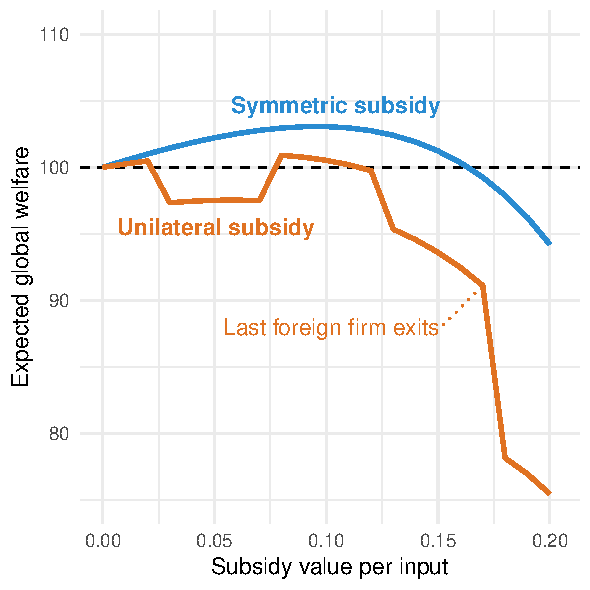
\includegraphics[width = \linewidth]{welfare.pdf}
        \\
        \small{Note: Calculated with same parameters as Table \ref{tab:input_subsidy}. Free trade case normalised to $\mathbb{E}(V) = 100$.} 
    \end{minipage}
\end{figure}

The third example, import tariffs on inputs, is shown in Table \ref{tab:input_tariff}. Tariff rates of 0.1 and 0.2 are chosen to illustrate the prisoner's dilemma dynamic. For the smaller tariff, welfare in the tariff-imposing country rises, and the Nash equilibrium is symmetrical small tariffs that reduce production and global welfare. Variance of supply and the shortage probability are not improved by tariffs.

One interesting result is the reduction in shortage probabilities under tariffs in columns 2 and 5, even though variation is unchanged and average supply is lower than in the free trade case. This result is an artefact of the number of firms and the chosen threshold for defining a shortage, which is half of expected free-trade output. Under free trade, if any two firms are disrupted, consumption will drop by about half, since there are four firms in total. Under small tariffs, if two firms are disrupted, but it is the two foreign firms, consumption will fall by less than half, since foreign firms now make up less than half of expected consumption. In column 3, variation is reduced because another firm enters in the tariff-imposing country. This outcome would not occur in equilibrium---under symmetric tariffs, shortage probability rises back to the free-trade level.

\begin{table}
    \centering
    \begin{threeparttable}
        \renewcommand{\arraystretch}{1.2}
        \caption{Input tariff example}
        \label{tab:input_tariff}
        \vspace{1mm} 
        \begin{tabular}{lrrrrr}
            \toprule
            & \multicolumn{5}{c}{Ad valorem tariff rate on inputs} \\
            & \makecell[c]{None} & \multicolumn{2}{c}{Unilateral} & \multicolumn{2}{c}{Symmetric} \\
            \cmidrule{2-2} \cmidrule{3-4} \cmidrule{5-6}
            & $t_A = 0$ & $t_A = 0.1$ & $t_A = 0.2$ & $t_A = 0.1$ & $t_A = 0.2$ \\
            & $t_B = 0$ & $t_B = 0$ & $t_B = 0$ & $t_B = 0.1$ & $t_B = 0.2$\\
            \midrule
            \textbf{Country A} \\
            Input producers & 2 & 2 & 3 & 2 & 2 \\
            $\mathbb{E}(V_A)$ & 20.05 & 20.64 & 19.02 & 19.95 & 19.72 \\
            $\mathbb{E}(Q_{IA})$ & 19.66 & 21.03 & 21.99 & 19.29 & 19.19 \\
            $\mathbb{E}(Q_{FA})$ & 23.25 & 20.97 & 19.42 & 22.46 & 21.92 \\
            $\mathbb{E}(X_{FA})$ & 15.80 & 15.44 & 15.21 & 15.26 & 14.89 \\
            $CV(X_{FA})$ & 17.50\% & 17.73\% & 15.40\% & 17.51\% & 17.43\% \\
            $\mathbb{P}(\text{Shortage})$ & 2.00\% & 1.18\% & 0.84\% & 2.02\% & 1.19\% \\ 
            \midrule
            \textbf{Country B} \\
            Input producers & 2 & 2 & 2 & 2 & 2 \\ 
            $\mathbb{E}(V_B)$ & 20.05 & 19.34 & 18.91 & 19.95 & 19.72 \\
            $\mathbb{E}(Q_{IB})$ & 19.66 & 17.95 & 16.91 & 19.29 & 19.19 \\
            $\mathbb{E}(Q_{FB})$ & 23.25 & 24.80 & 25.90 & 22.46 & 21.92 \\
            $\mathbb{E}(X_{FB})$ & 15.80 & 15.66 & 15.58 & 15.26 & 14.89 \\
            $CV(X_{FB})$ & 17.50\% & 17.52\% & 15.40\% & 17.51\% & 17.43\% \\
            $\mathbb{P}(\text{Shortage})$ & 2.00\% & 1.18\% & 0.84\% & 2.02\% & 1.19\% \\ 
            \midrule
            \textbf{Country C} \\
            $\mathbb{E}(V_C)$ & 17.73 & 17.44 & 17.25 & 17.13 & 16.72 \\
            $\mathbb{E}(X_{FC})$ & 14.91 & 14.68 & 14.53 & 14.41 & 14.06 \\
            $CV(X_{FC})$ & 17.49\% & 17.61\% & 15.36\% & 17.46\% & 17.35\% \\
            $\mathbb{P}(\text{Shortage})$ & 2.00\% & 1.18\% & 0.84\% & 2.02\% & 2.00\% \\ 
            \midrule
            \textbf{All countries} \\
            Input producers & 4 & 4 & 5 & 4 & 4 \\
            $\mathbb{E}(V)$ & 57.82 & 57.42 & 55.17 & 57.03 & 56.16 \\
            $\mathbb{E}(Q_I)$ & 39.32 & 38.97 & 38.90 & 38.57 & 38.38 \\
            $\mathbb{E}(Q_F)$ & 46.50 & 45.77 & 45.32 & 44.93 & 43.84 \\
            $CV(Q_F)$ & 17.49\% & 17.61\% & 15.36\% & 17.46\% & 17.35\% \\
            $\mathbb{P}(\text{Shortage})$ & 2.00\% &1.18\% & 0.84\% & 2.02\% & 2.00\% \\ 
            \bottomrule
        \end{tabular}
        \begin{tablenotes}
            \small \item Note: Calculated with $p_R = 0.5$, $\sigma = 5$, $\tau = 0.1$, $\kappa = 1$ and $d_A = d_B = 0.1$. Income for all countries is set to 10. Variation and probability are based on 30 samples of 20,000 simulations each. Bootstrap standard errors all $<0.01\%$.
        \end{tablenotes}
    \end{threeparttable}
\end{table}

The fourth example is an export ban on inputs, shown in Table \ref{tab:export_ban}. Because there are only two producing countries, a ban of exports from Country $A$ is equivalent to a 100 per cent local content requirement for Country $B$'s final sector. Simulating the model with export bans requires a modification to prices. Since producers in $B$ can no longer access inputs in $A$, their production technology becomes less efficient---one of the input quantities in \ref{eq:prod_final} is set to zero---and their unit cost becomes equal to the price of inputs from their own country $p_{IB}$. Given perfect competition, the price of final goods changes to match this unit cost. Firms in the input sector anticipate this change when considering entry.

Any export ban reduces expected welfare for all three countries. Behind this unsurprising result, there are some nuances. When country $A$ alone bans exports of inputs, its domestic production of inputs grows, perhaps counterintuitively. Because $B$ can no longer source foreign inputs, its production of final goods becomes much less efficient, causing $A$'s share of global final goods production to rise (in this example, to 65 per cent). To meet this greater demand, a new firm enters in $A$, but conditions are not yet bad enough for a firm in $B$ to drop out, resulting in more firms making fewer goods---and lower supply variation because risk is spread more widely. An extension would be to incorporate country-specific risk, not just firm-specific risk, and check if this type of result is still feasible.

An implication of this result is that, if countries act solely to minimise variation or shortage probability for a critical final good, then under certain conditions, there will be a coordination failure. It is less `prisoner's dilemma' and more `game of chicken': the example in Table \ref{tab:export_ban} implies a mixed strategy Nash equilibrium with a higher expected probability of a shortage than would be the case under free trade. This makes the case for a trade agreement on risk-reducing grounds alone. If reducing shortage risk is not an objective, however, and only average welfare matters, export bans do not eventuate in this model.

\begin{table}
    \centering
    \begin{threeparttable}
        \renewcommand{\arraystretch}{1.2}
        \caption{Input export ban example}
        \label{tab:export_ban}
        \vspace{1mm} 
        \begin{tabular}{lrrr}
            \toprule
            & \multicolumn{3}{c}{Export-banning country} \\
            \cmidrule{2-4}
            & \makecell[c]{Neither} & \makecell[c]{$A$} only & \makecell[c]{$A$ and $B$} \\
            \midrule
            \textbf{Country A} \\
            Input producers & 2 & 3 & 2 \\ 
            $\mathbb{E}(V_A)$ & 20.05 & 18.82 & 17.77 \\
            $\mathbb{E}(Q_{IA})$ & 19.66 & 25.46 & 20.41 \\
            $\mathbb{E}(Q_{FA})$ & 23.25 & 28.99 & 20.41 \\
            $\mathbb{E}(X_{FA})$ & 15.80 & 15.45 & 13.87 \\
            $CV(X_{FA})$ & 17.50\% & 15.29\% & 17.13\% \\
            $\mathbb{P}(\text{Shortage})$ & 2.00\% & 0.37\% & 4.46\% \\ 
            \midrule
            \textbf{Country B} \\
            Input producers & 2 & 2 & 2 \\
            $\mathbb{E}(V_B)$ & 20.05 & 18.43 & 17.77 \\
            $\mathbb{E}(Q_{IB})$ & 19.66 & 18.52 & 20.41 \\
            $\mathbb{E}(Q_{FB})$ & 23.25 & 15.36 & 20.41 \\
            $\mathbb{E}(X_{FB})$ & 15.80 & 14.67 & 13.87 \\
            $CV(X_{FB})$ & 17.50\% & 15.55\% & 17.12\% \\
            $\mathbb{P}(\text{Shortage})$ & 2.00\% & 1.60\% & 4.45\% \\ 
            \midrule
            \textbf{Country C} \\
            $\mathbb{E}(V_C)$ & 17.73 & 16.75 & 15.57 \\
            $\mathbb{E}(X_{FC})$ & 14.91 & 14.23 & 13.09 \\
            $CV(X_{FC})$ & 17.49\% & 15.30\% & 16.68\% \\
            $\mathbb{P}(\text{Shortage})$ & 2.00\% & 0.86\% & 5.26\% \\ 
            \midrule
            \textbf{All countries} \\
            Input producers & 4 & 5 & 4 \\
            $\mathbb{E}(V)$ & 57.82 & 54.00 & 51.11 \\
            $\mathbb{E}(Q_I)$ & 39.32 & 43.97 & 40.83 \\
            $\mathbb{E}(Q_F)$ & 46.50 & 44.35 & 40.83 \\
            $CV(Q_F)$ & 17.49\% & 15.30\% & 16.68\% \\
            $\mathbb{P}(\text{Shortage})$ & 2.00\% & 0.86\% & 5.26\% \\ 
            \bottomrule
        \end{tabular}
        \begin{tablenotes}
            \small \item Note: Calculated with $p_R = 0.5$, $\sigma = 5$, $\tau = 0.1$, $\kappa = 1$ and $d_A = d_B = 0.1$. Income for all countries is set to 10. Variation and probability are based on 30 samples of 20,000 simulations each. Bootstrap standard errors all $<0.01\%$.
        \end{tablenotes}
    \end{threeparttable}
\end{table}

\section{Towards principles for supply chain resilience policy}

In a highly stylised setting, the last section demonstrated some mechanisms through which different industrial policies might affect the performance and resilience of supply chains, domestically and internationally. Turning to active policy proposals, economic research to date suggests there are a few rules of thumb for domestic and international policymakers with the objective of supply chain resilience.

First, at a domestic level, industrial policies aimed at improving supply chain resilience should be designed to support competition and avoid raising unnecessary barriers for new entrants. Empirical work on industrial policy in Japan and China supports this conclusion on productivity grounds \parencite{porter_competition_2004, aghion_industrial_2015}. From a theoretical perspective, a competitive environment domestically means risk is spread more broadly and the persistence of bottlenecks is less likely.

To enhance resilience, policymakers might favour policy instruments that encourage firm entry, while recognising that in some cases, there may be large trade-offs between resilience and productivity. (\textcite{barwick_chinas_2019}, for example, found that entry subsidies in China's shipbuilding sector made idleness and productivity issues worse, partly because of the industry's economies of scale.) Such instruments might include temporary tax incentives for new entrants, expanded R\&D incentives, or streamlined regulatory processes for sectors identified as vulnerable and essential. These measures can help diversify the supplier base and reduce dependency on a limited number of sources.

Second, the range of available policy instruments is broad and the right tool depends on the task at hand. For example, if seeking to ensure the reliable supply of a critical product, purchasing from a diverse portfolio of global and local suppliers might be more cost effective than investing commensurately in domestic production capacity, depending on the sector. An emphasis on measurement and evaluation of these policies seems essentially 'no regrets' and would generate useful data.

Third, as the \textcite{productivity_commission_vulnerable_2021} point out, a focus on essential and vulnerable sectors is crucial when supply chain resilience is the primary goal. These sectors are the nexus in which there is most likely to be a gap between private risk management outcomes and public risk tolerances.

Internationally, improving data collection on industrial policies and modelling their positive and negative spillovers is an important and rapidly growing space for researchers and policymakers. Tasking an organization with existing capacity in the area, such as the OECD, IEA, WTO, or potentially IPEF in the future, with independently reporting on essential supply chains and identifying vulnerabilities could provide valuable insights for policymakers globally. A recent IEA report, for example, points to alarming levels of concentration in PV wafer production and makes a brief, convincing case for intervention to alleviate it \parencite{iea_solar_2022}.

The question of whether and how the world trading system should address supply chain risk hinges at least as much on political and geopolitical contingencies than it does on economic welfare. The section above and conventional economic wisdom suggest that upstream export bans and local content requirements are generally inefficient means of attaining a secure supply. These measures already violate WTO rules. The European Union notably brought a case against Indonesia's raw materials export bans with both China and the United States joining as third parties, a case which is under appeal as of 2024.

Greater political buy-in is needed to adequately discourage these policies, probably via plurilateral arrangements and in exchange for accommodating other, less distorting (or indeed, net-beneficial) policies. To that end, developing and reinforcing guardrails against policies that remove sources of supply will be important if the performance and stability of GVCs is an objective. This could include restrictions on export bans outside of immediate critical shortages, such as food shortages, ensuring that countries do not exacerbate supply chain disruptions through unilateral actions. Since some export restrictions are inevitable on defence grounds, a negative-list approach to restrictions would be the way forward to minimise certainty.

Following the model of the WTO Agreement on Agriculture, and as suggested by scholars like \textcite{aguayo_ayala_preserving_2005} and \textcite{bown_wtoing_2019}, promoting a `green, amber, red light' approach in the WTO could help manage supply chain-related policies more effectively. For example, policies that introduce a new source of supply for an extremely concentrated product---like PV wafers---using acceptable instruments could be classified as `green light', indicating their general acceptability within world trade rules.

\section{Concluding remarks}

This paper explores the theoretical grounds, current implementation and international governance of industrial policies aimed at improving supply chain resilience. Through a simple three-country model, we illustrate potential spillovers from various policy instruments, including entry subsidies, production subsidies, import tariffs and export bans. Since numerical methods are used here, a low-hanging area for future research would be to attempt to formalise the key conclusions. The model could also be generalised to include many countries, many stages of production, or non-CES preferences, as \textcite{grossman_supply_2023} suggest. Supply chain resilience is an increasingly prominent topic for scholars and policymakers, and exploring the implications of new findings for international cooperation seems a particularly pressing need.

\nocite{dcceew_department_of_climate_change_energy_the_environment_and_water_securing_2022}

\printbibliography

\end{document}